\chapter{Estrategia de resolución}

En este capítulo se explica el proceso llevado a cabo para desarrollar la solución. La metodología se basa en tres puntos, estos son: el modelado del problema, el algoritmo genético desarrollado y la simulación del trafico.

Se presenta el modelado del problema, el proceso de simulación y el algoritmo genético utilizado con su estructura, parámetros y configuración. Se detalla la biblioteca utilizada para el desarrollo del algoritmo genético y la arquitectura propuesta.


\section{Modelado del problema }

Para solucionar el problema se usarán simulaciones de la realidad, por tanto es importante contar con un modelo detallado y fidedigno. A continuación se da información sobre el simulador a utilizar, las herramientas necesarias y el proceso seguido para generar el modelo. 

\subsection{Simulador SUMO (Simulation of Urban MObility)}

Como se explicó en el marco teórico SUMO es un simulador de tráfico gratuito y abierto que nos permite modelar redes de calles, vehículos, transporte público, ciudadanos y semáforos. Sigue un modelo microscópico ya que realiza la simulación individual explícita de cada elemento. Incluye un conjunto de herramientas destinadas  a facilitar la generación de tráfico y la construcción de mapas. 

Dado que existe un amplio abanico de posibilidades a la hora de elegir un simulador se efectuó un análisis relacionado a las posibilidades y objetivos del proyecto. Las siguientes son las razones que sustentan la elección de SUMO como el simulador utilizado:

\begin{itemize}
	\item Portable: SUMO puede ser ejecutado tanto en Windows como en Linux, lo cual es importante dado que son las plataformas en las que se desarrolla el proyecto y Linux (CentOs) es el sistema operativo utilizada por el Cluster Fing en donde se ejecutará el algoritmo..
	
	\item Tipos de ejecución: Permite las opciones de ejecutarse sin interfaz gráfica utilizando la línea de comando lo que aumenta sensiblemente la velocidad de ejecución. Esto es fundamental a la hora de realizar la arquitectura necesaria ya que el programa tiene que tener la posibilidad de ejecutar el simulador de manera directa. Por otro lado también tiene la opción de mostrar la interfaz gráfica lo cual es indispensable a la hora de visualizar la simulación, sobre todo en los primeros momentos del desarrollo en los cuales se realizan ajustes y pruebas.
	
	\item Gratuito y abierto: SUMO es de código abierto y sin costo, el cual es un factor importante para un proyecto de investigación, como el que se quiere desarrollar. 
	
	\item Documentación y mantenimiento: Cuenta con una detallada documentación lo cual hace más fácil su utilización, así como una comunidad muy activa que responde dudas en foros lo cual es útil a la hora de buscar soporte si ocurriera algún problema o se detectara un error. También cuenta con un desarrollo activo lo cual es importante pues se realizan correcciones y actualizaciones frecuentemente.
	
	\item Configuración simple: Tiene un sistema sencillo para configurar las simulaciones basada en archivos XML. Pudiendo de esta forma modificar la configuración de los semáforos, las propiedades de los vehículos, las rutas que estos siguen entre otras opciones. Además tiene herramientas para poder utilizar mapas importados de servicios como \citet{OSM}.
	
	\item Información de salida: SUMO tiene la opción de generar una amplia gama de datos producto de la simulación entre los que se encuentran la velocidad de los vehículos y el largo del recorrido, datos requeridos por la solución propuesta.
	
	\item Eficiente: Soporta redes de tránsito muy grandes y está diseñado para ejecutar simulaciones a gran velocidad \citep{sumo2014}, lo cual es una característica deseable por la complejidad del problema a solucionar.
	
\end{itemize}


SUMO tiene un funcionamiento sencillo basado en tomar como entradas archivos de configuración que representan la red vial, los vehículos, el tráfico y los semáforos. También genera archivos de salida con información interesante como el tiempo de simulación, la cantidad de vehículos, sus velocidades, duración del viaje, emisiones de gases contaminantes, etc. 

Dada la complejidad del problema a enfrentar, se utilizaron otras herramientas útiles para que ciertas tareas fueran realizadas de manera más eficiente y con menos errores. \emph{NetConvert} viene integrado con SUMO y fue utilizado para la generación de la red vial a partir del mapa obtenido de Open Street Map, transformándolo al formato que SUMO reconoce. Otra herramienta integrada con SUMO es \emph{DUaRouter} que permite generar recorridos de vehículos basado en dinámicas definidas por el usuario. \emph{Traffic Modeler} creado por \citet{TrafficModeler}, es útil para la generación de tráfico de manera visual y puede ser exportado para que sea reconocido por SUMO. 
	


\begin{figure}[H]
	\centering
	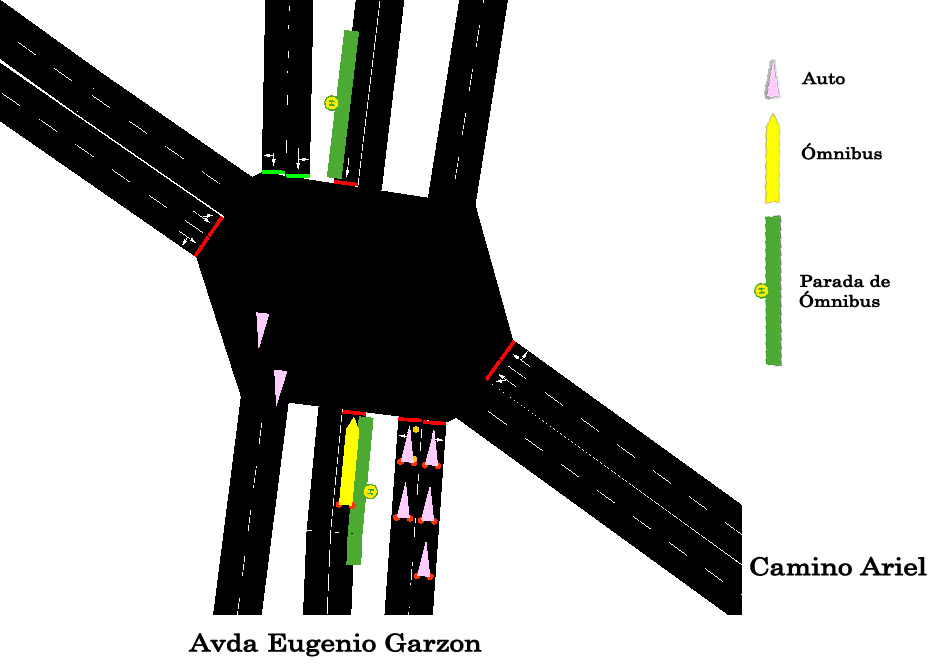
\includegraphics[width=0.7\linewidth]{Figures/sim1}
	\caption{Simulacion de tráfico en SUMO en el cruce entre Bulevar Battle y Ordoñez y el Corredor Garzón.}
	\label{fig:sim1}
\end{figure}



\subsection{Proceso del modelado}

Se describen los pasos realizados para tener los elementos necesarios para ejecutar la simulación.

\subsubsection{Diseño del mapa}

El primer paso consiste en desarrollar un mapa de la zona que sea compatible con el simulador. Para ello se utiliza el servicio de Open Street Map \citep{OSM} que cuenta con mapas libres y actualizados por una comunidad muy activa. Se importa la zona de interés del mapa al editor \citet{JOSM} para poder adecuarlo a las necesidades del problema. 

El alcance que se pretende es la zona que corresponde al Corredor Garzón desde su inicio hasta el final y dos caminos paralelas a cada lado.
Como se ve en el mapa de la figura \ref{fig:mapa_osm_sumo}, no existen calles paralelas reales, por lo que se eligieron primero las calles que corresponderían a las paralelas y todas las calles que permiten ir de una de las calles paralelas a otra. Luego se verifica que cada paralela se constituya por una calle doble mano o dos calles de una sola mano y luego se borraron manualmente todas las demás calles.

Al notar que habían calles de una sola mano que estaban representadas en Open Street Map como doble vías y que algunos cruces de Garzón como Lezica diferían con lo visto in situ, se modificaron los datos importados. Se utilizaron otros servicios como Google Maps y Bing Maps como consulta ya que al poseer mapas y fotos actualizadas del lugar se podía discernir y recordar como eran exactamente las calles en la actualidad. Como el paso previo fue la eliminación de las calles que no fueran las paralelas, no se podían subir los cambios realizados (porque desaparecerían calles que realmente existen) y por este motivo no se pudo contribuir a la comunidad actualizando el mapa de OSM.

\begin{figure}[H]
	\centering
	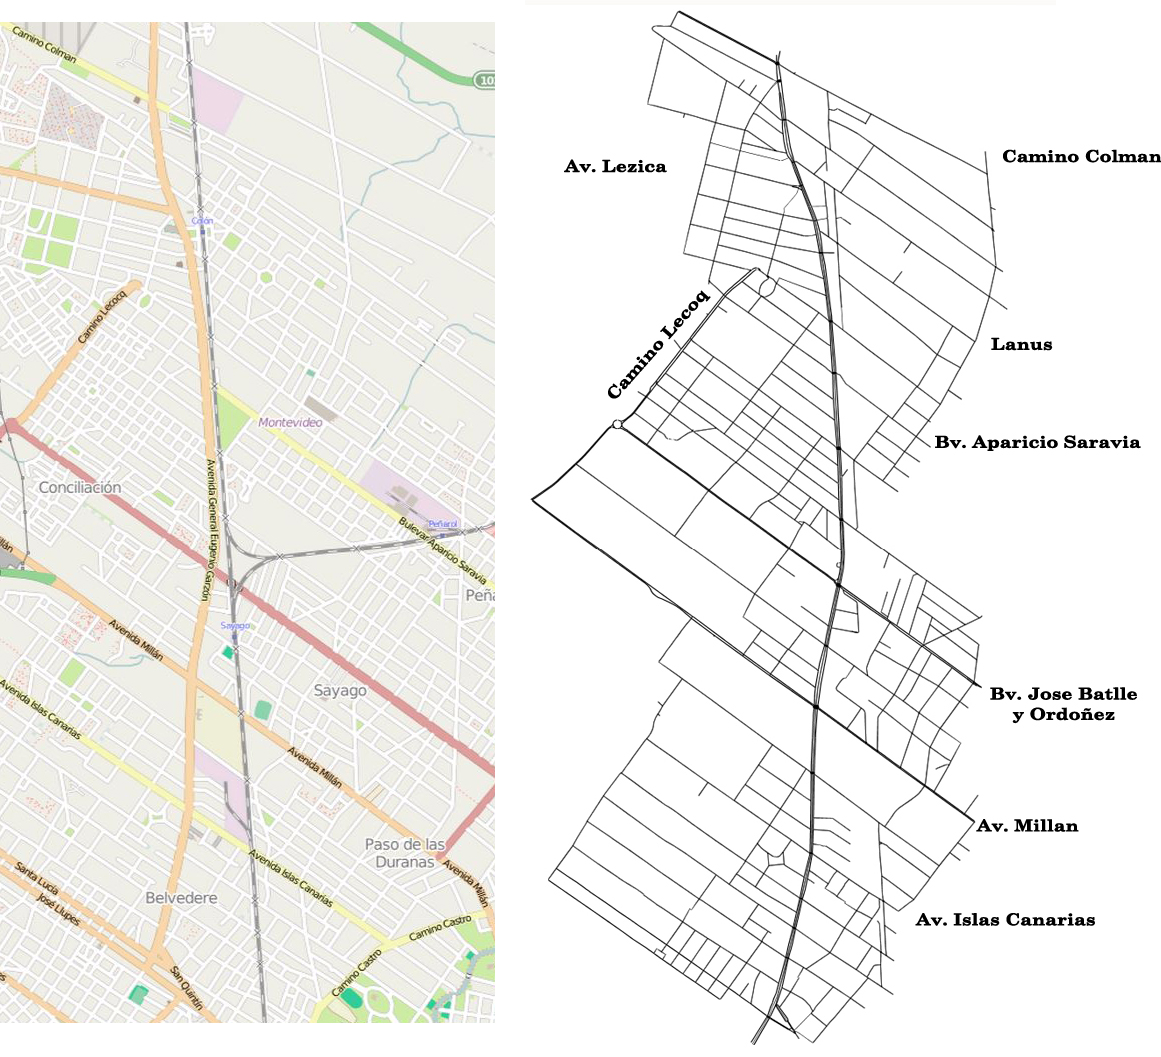
\includegraphics[width=0.9\linewidth]{Figures/mapa_osm_sumo}
	\caption{A la izquierda el mapa extraído de OSM, a la derecha el mapa procesado listo para ser usado en SUMO. El corredor Garzón está en el centro de cada imagen.}
	\label{fig:mapa_osm_sumo}
\end{figure}

Se utilizó la herramienta Netconvert para transformar el formato OSM al formato XML que SUMO reconoce. Netconvert no reconoce muchos de los datos aportados por el formato OSM como los números de las casas, las vías del tren, las vías de peatones, los caminos, las plazas, las paradas y los separadores que tiene el corredor de las vías de autos, entre muchos otros. Pero lo mas importante es que no funciona correctamente para reconocer corredores, por lo que mezclaba y superponía el corredor central con las vías de los autos, esto seguramente por no reconocer los separadores físicos que tiene el corredor. 

Primero se filtraron y borraron todos los datos que no eran reconocidos por NetConvert mediante la eliminación de elementos por etiquetas que permite el 
JOSM. Luego se separaron aproximadamente un metro las calles de él corredor central. Si bien esto logró que NetConvert interpretara que no era posible cambiar entre la vía de los autos y la del corredor de ómnibus, también generó un error ya que cada cruce de la realidad era tratado como tres cruces distintos (uno por cada calle del corredor).

Finalmente se realizaron varios ajustes confeccionando manualmente archivos xml para que lo generado por el NetConvert corrigiera todos los errores que genera por defecto. Los distintos cruces con múltiples semáforos antes mencionados se manejan con la unión de nodos. La falta de las prohibiciones de los virajes a la izquierda que presentaba se corrigió con un archivo de las conexiones posibles.

Siguiendo estos pasos se obtuvo un mapa fiel a la realidad y compatible con el simulador.


\subsubsection{Trabajo de campo}
Se cuentan con los datos públicos sobre la cantidad de  ómnibus y sus frecuencias pero no se tienen datos sobre la densidad de tráfico vehicular en la zona, por esto se realizó un revelamiento in-situ con las siguientes características.

Se seleccionaron cinco cruces que presentan diferentes características para poder modelar variantes en la cantidad de vehículos circulantes.
Estos son: Camino Ariel, Battle y Ordoñez, Plaza Videla, Camino Colman y Aparicio Saravia. 

Se siguen las recomendaciones de los textos consultados al respecto \citep{ConteoTrafico}. Se eligió el día miércoles, que estuviera soleado y entre las 15 y 17 horas para no tener los sesgos que se producen los fines de semana o días de lluvia.
Se realizaron filmaciones de entre 15 y 30 minutos en los cruces y luego se analizaron los vídeos para realizar el conteo manual con la posibilidad de enlentecer el vídeo para mayor facilidad. Luego se completa una planilla electrónica (figura \ref{fig:conteo_hoja}) donde se tiene la información de vehículos que recorren Garzón, la calle que cruza y los que doblan. 

\begin{figure}[H]
	\centering
	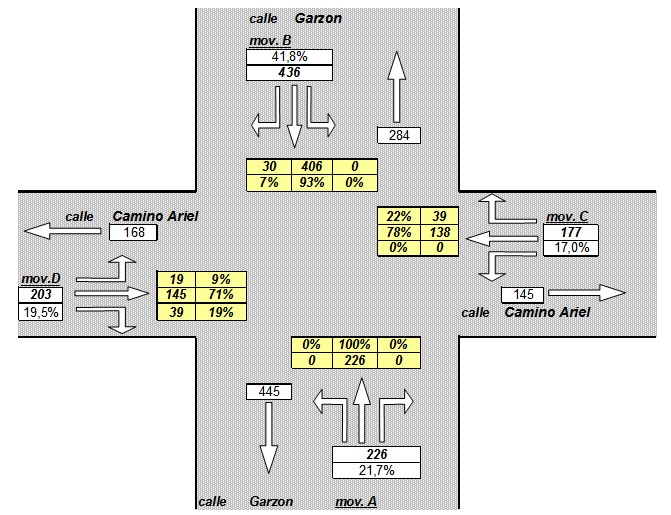
\includegraphics[width=0.9\linewidth]{Figures/conteo_hoja}
	\caption{Ejemplo de planilla electrónica para el conteo manual en Camino Ariel}
	\label{fig:conteo_hoja}
\end{figure}



\begin{table}[H]
	\renewcommand{\arraystretch}{1.2}
	\caption{Resumen del revelamiento del tráfico en la zona del corredor Garzón. Se muestra la cantidad de vehículos y la orientación hacia donde circulan.}
	\label{table:resumen_trafico}
	\centering
	\begin{tabular}{lcccc}
		\hline
		Intersección&
		Sur-Garzón& 
		Norte-Garzón & 
		Oeste &
		Este 
		\\ 
		\hline
		Camino Colman  & 410 & 390 & 140 & 230\\		
		Plaza Vidiella  & 400 & 444 & 292 & 0\\		
		Aparicio Saravia  & 390 & 450 & 40 & 90\\		
		Battle y Ordoñez  & 510 & 390 & 470 & 300 \\	
		Camino Ariel  & 436 & 226 & 177 & 203 \\													
		\hline
		
		
		\hline
	\end{tabular}
\end{table}

En la tabla \ref{table:resumen_trafico} se muestra la cantidad de vehículos en los distintos cruces; hay que tener en cuenta que solo se contabilizan autos, no se tienen en cuenta otro tipo de vehículos.

Además se realizaron recorridas de punta a punta del corredor a una velocidad constante en auto para verificar los tiempos obtenidos de la simulaciones.

Para la configuración de los semáforos se realizó un recorrido en bicicleta por el corredor cronometrando la duración del tiempo en cada esquina de cada semáforo, tanto de ida como de vuelta para corroborar que fueran correctos. Estos tiempos fueron verificados por los vídeos obtenidos.



\subsubsection{Modelo del tráfico}
Una vez que se tiene el mapa compatible con el simulador y los datos relevados de la realidad, se agrega el tráfico a la simulación.

Existen varios modelos disponibles para representar la circulación de los vehículos. El modelo \emph{aleatorio} genera diferentes recorridos que seguirán los vehículos aleatoriamente. En el modelo \emph{basado en áreas} se especifican diferentes áreas que indican los lugares en donde el tráfico se origina y donde finaliza. Otro modelo mas complejo es el \emph{basado en actividad} donde se especifica la cantidad de casas, vehículos y población en un determinado lugar y el modelo genera la densidad de tráfico que se producirá basado en los tipos de actividades que se realizan comúnmente como ir al trabajo, hacer las compras, ir a la escuela, etc. Otro modelo muy utilizado sobre todo en escenarios de tamaño reducido es el \emph{definido por el usuario} que permiten determinar la ruta de cada vehículo con mayor detalle.

Se utilizó el programa Traffic Modeler \citep{TrafficModeler} que sirve para generar modelos de tráfico complejos de manera visual. Se optó por un modelo de movilidad entre áreas lo que permite una buena granularidad al especificar la densidad de tráfico. Esto genera el recorrido del viaje para cada vehículo, los mismos se mantienen constantes en las distintas ejecuciones del algoritmo. La variación se da en las velocidades desarrolladas por cada uno, ya que dependiendo de la configuración de los semáforos logrará mayores o menores velocidades.



\begin{figure}[h]
	\centering
	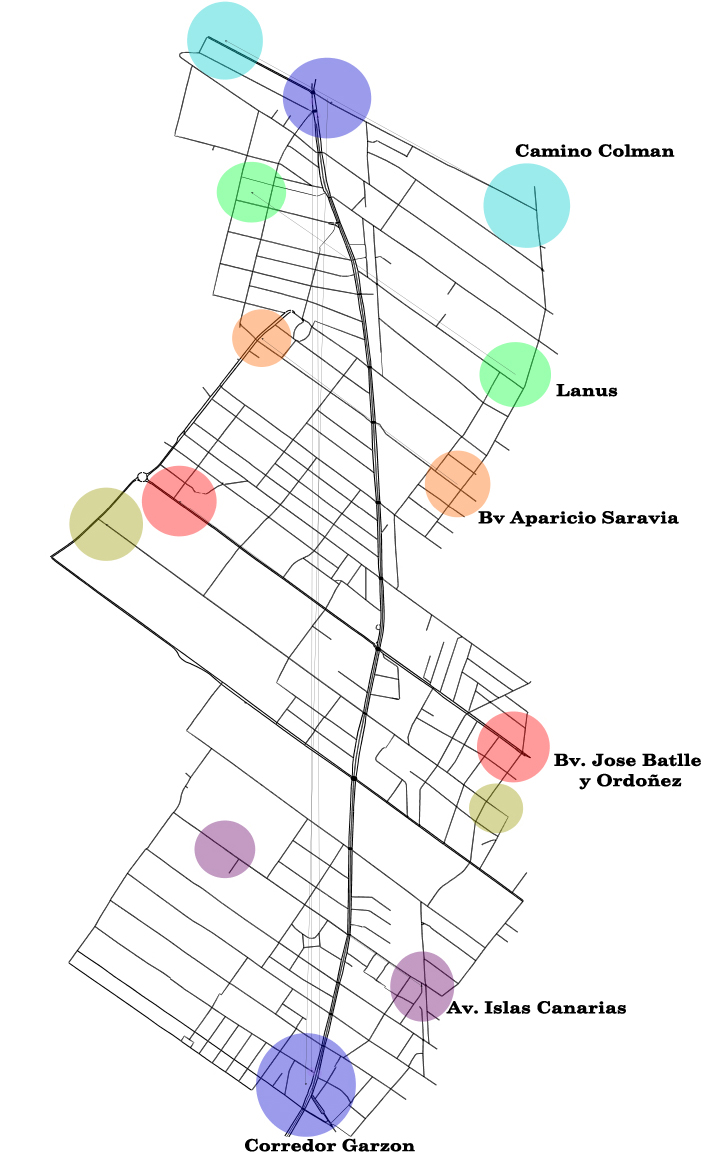
\includegraphics[width=0.4\linewidth]{Figures/areaflow1}
	\caption{Mapa del TrafficModeler con las áreas de tráfico. Círculos del mismo color indican tráfico especificado entre esas áreas}
	\label{fig:areaflow1}
\end{figure}


Se manejaron dos tipos de vehículos autos y ómnibus cada uno con características distintas tanto de tamaño, aceleración y velocidad máxima. No se especifican otros tipos de vehículos como motos o camiones ya que el trabajo se enfoca en los dos primeros tipos.

Se agregaron las frecuencias y los distintos recorridos de los ómnibus obtenidos de datos públicos de la Intendencia Municipal de Montevideo \citep{IMM}. Estos incluyen las líneas urbanas  'G', '409' ,'2', 'd5'  y  '148'. Las líneas de ómnibus suburbanas realizan  un mismo  trayecto y se generalizan con el nombre 'A' las cuales no van a ser tomadas en cuenta en la optimización del algoritmo pero si aparecerán en la simulación.

La ubicación y líneas de cada parada se obtuvo de \citep{sigMontevideo}. Existen 14 paradas de líneas urbanas por el corredor para el recorrido de ida y la misma cantidad para la vuelta. Para los recorridos se hicieron  variantes  en  los  viajes  dentro  de  una  misma línea para simular el hecho de que no siempre se para en las mismas paradas. También se tuvo en cuenta para la simulación el tiempo que demora un ómnibus al detenerse en una parada y que hay algunas donde por la cantidad de gente se demora más. Estos datos fueron obtenidos en el lugar considerando tiempos de entre 15 a 35 segundos.

Se realizó un estudio basado en datos de GPS proporcionados por la IMM. Estos datos cuentan con la posición exacta en coordenadas geográficas, la velocidad instantánea y la referencia del ómnibus para un conjunto de líneas seleccionadas tomadas en un período de una semana. 
Para este procesamiento fue necesario utilizar QGIS, un sistema de información geográfico capaz de visualizar, editar y realizar operaciones sobre elementos geográficos. Además se desarrollaron \emph{scripts} para obtener las estadísticas necesarias ya que la cantidad de información estudiada era muy grande (1.5Gb). Esto permitió seleccionar, filtrar y relacionar los datos de posición y velocidad con las líneas que circulan por el Corredor Garzón. Luego de procesar los datos se obtuvo una velocidad media es de 14.5 km/h lo que permite ajustar mejor el modelo. 

Para configurar la simulación se utilizan como entrada tres archivos de configuración en formato XML que son reconocidos por el simulador SUMO. El primero es el archivo de \emph{configuración de los semáforos} donde se detalla su duración, el comienzo de fase y la ubicación de los mismos en el mapa base. El segundo es el archivo con la \emph{ruta de los vehículos} que contiene el recorrido de cada vehículo. Finalmente el archivo con el \emph{recorrido de los ómnibus} que indica el recorrido de los mismos, su frecuencia, la ubicación de las paradas, en cuales se detienen y cuanto demoran en la parada.

\section{Arquitectura de la solución}

En la figura \ref{fig:arquitectura1} se muestra la arquitectura propuesta para el problema.

La biblioteca Malva se utiliza para la implementación del algoritmo. En cada evaluación de la función de fitness se realiza un llamado al simulador SUMO. 

En el primer paso el algoritmo genera la población inicial, estos individuos representan una configuración de semáforos para el Corredor con el tiempo de duración de las luces y las fases. Esta población se genera realizando algunas variaciones de los valores reales obtenidos.

\begin{figure}[H]
	\centering
	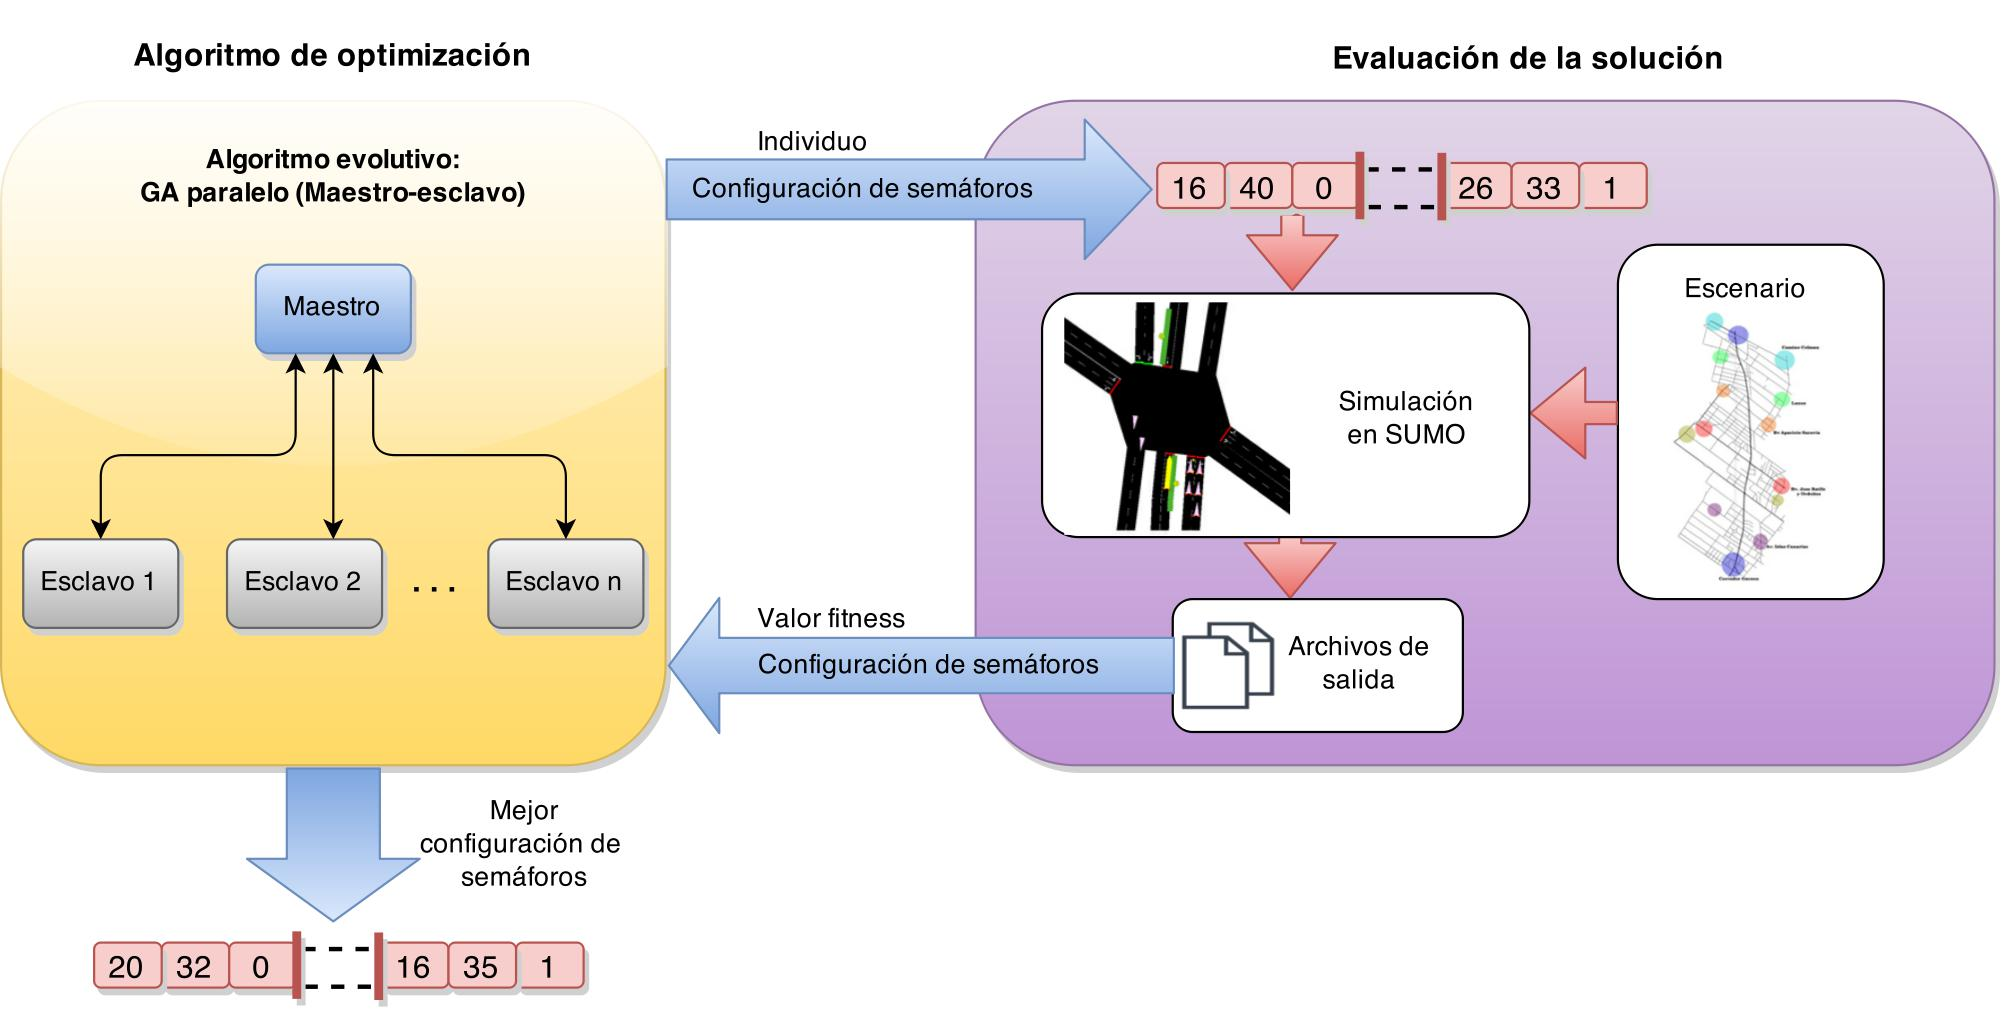
\includegraphics[width=0.7\linewidth]{Figures/arquitectura1}
	\caption{Arquitectura de la función de fitness}
	\label{fig:arquitectura1}
\end{figure}

Luego por cada individuo se genera un archivo compatible con el simulador que representa la configuración de semáforos. Este archivo se utiliza como entrada para ejecutar el simulador para cada individuo. Al finalizar la ejecución se generan archivos de salida que son procesados por el algoritmo, estos tienen la información necesaria para calcular el fitness de cada individuo como la velocidad media de ómnibus y otros vehículos.

El algoritmo se detiene al alcanzar un número de generaciones determinado en ese momento se crea un archivo que tiene la mejor configuración de semáforos encontrada.




\section{Implementación: Biblioteca Malva}

Dada la complejidad del problema se tuvo en cuenta desde un inicio la utilización de un \emph{framework}, de esta forma se podría lograr una ejecución eficiente y una implementación robusta pero flexible. 

Como se detalló en el marco teórico existen varias opciones de \emph{frameworks} disponibles. Por las particularidades del problema existen ciertos requerimientos a la hora de seleccionar  uno para su resolución, entre los que se destacan:

\begin{itemize}
	\item Abierto y gratuito: Al ser un proyecto de investigación de índole académico es conveniente que no se tengan costos económicos asociados. Además es importante que se cuente con el código abierto con el fin de introducir modificaciones en el código base o corregir errores.
	\item Algoritmo genético: El \emph{framework} debe facilitar el desarrollo de un algoritmo genético ya que es la base en la que se sustenta el proyecto.
	\item Algoritmo paralelo: Por la complejidad del problema y el alto consumo de recursos computacionales que insume, es fundamental la opción de ejecución en paralelo. Si no cuenta con funcionalidad nativa al menos que tenga la posibilidad de modificar el código principal para agregarlo.
	\item Plataforma: Es requerido que se pueda ejecutar en el Cluster Fing (CentOs - Linux), en Windows y otros sistemas Linux, ya que son las plataformas en donde se desarrollará el trabajo.
	\item Confiabilidad: Es deseable que sea lo suficientemente estable como para tener confianza de que el algoritmo funcionará sin demasiados problemas de manera correcta. Por ejemplo que existan casos de éxito usando el \emph{framework}, documentación, ejemplos de código, etc.
	\item Lenguaje: Es deseable que esté desarrollado en C++ o Java por la experiencia que se cuenta en estos lenguajes. 
	\item Multiobjetivo: Es deseable (aunque no requerido) que soporte algoritmos multiobjetivo, ya que la función que se quiere implementar aún siendo multiobjetivo es sencilla.	
\end{itemize} 

Luego de analizar todos estos puntos se selecciona la biblioteca Malva para la implementación del algoritmo. A continuación se detalla su funcionamiento y características.

Como se explicó anteriormente \citet{Malva} surge como una variante del proyecto \citet{Mallba}. Propone su actualización, mejora y desarrollo como un proyecto de código abierto colaborativo.  Su objetivo es proveer de varios esqueletos de heurísticas de optimización que puedan ser utilizados y extendidos de manera fácil y eficiente.

Los esqueletos se basan en separar dos conceptos: El problema concreto que se quiere resolver y por otro lado el método utilizado para resolverlo. Por tanto un esqueleto se puede ver como una plantilla genérica que se instancia para resolver un problema particular, manteniendo todas las funcionalidades genéricas.

Utiliza el lenguaje C++ dado su alto nivel, modularidad y flexibilidad. Los esqueletos se ofrecen como un conjunto de clases requeridas que son las que el usuario deberá modificar para adaptarlo a su problema y las provistas que incluyen todos los aspectos internos del esqueleto y son independientes del problema particular. Entre los algoritmos provistos se encuentra el de Algoritmos genéticos y \citet{CHC}.




\section{Modelo de paralelismo e implementación}

Uno de los requisitos planteados al inicio del presente trabajo era la creación de un algoritmo genético que soportara paralelismo con el objetivo de reducir los tiempos de ejecución del algoritmo ya que los escenarios planteados se consideraron complejos y que utilizarían gran cantidad de recursos computaciones. Para este propósito se utilizó como código base el algoritmo genético provisto por la biblioteca Malva llamado NewGA. A dicho código se le realizaron algunas modificaciones para lograr su ejecución en paralelo, específicamente se modificó la forma en que se evalúan los individuos generando un hilo de ejecución por cada individuo y distribuyendo la evaluación.
 
 Se utilizó el método maestro-esclavo donde el proceso maestro se encarga de la mayoría de las etapas del algoritmo. El maestro primero inicializa la población y se encarga de distribuir la evaluación de los individuos hacia los esclavos creando un hilo por cada esclavo. Luego espera a que las evaluaciones terminen para obtener los valores de \emph{fitness} de los esclavos. Una vez obtenidos, selecciona a los mejores individuos y le aplica los operadores de cruzamiento y mutación. Para finalizar aplica el operador de reemplazo para generar la siguiente población. Mientras los esclavos se encargan solamente obtener el individuo enviado por el maestro y de ejecutar la evaluación del individuo, que corresponde a ejecutar el simulador y obtener los datos de salida.
 
 En la sección de análisis experimental se realiza un estudio de la eficiencia computacional del algoritmo genético paralelo, para conocer comparar los tiempos de ejecución entre la versión paralela y en serie.

\section{Especificación del Algoritmo Genético utilizado}
Se utiliza el algoritmo genético provisto por la biblioteca  Malva  llamado NewGA con las modificaciones detalladas en la sección anterior. El siguiente esquema muestra el algoritmo utilizado:

\begin{algorithm}[H]
	\caption{Algoritmo Genético de Malva. }
	\label{alg:algoritmo_genetico_malva}
	\begin{algorithmic} [1] 
		{
			\STATE \texttt{t} = 0
			\STATE {Inicializo( P(t))}
			\STATE {Evaluar estructuras en ( P(t))}			
			\WHILE {\text{No termine}}
			\STATE \texttt{t}++		
			\STATE {Seleccionar C(t) de P(t-1)}	
			\STATE {Recombinar estructuras en C(t) formando C'(t)}				
			\STATE {Mutar estructuras en C'(t) formando C''(t)}		
			\STATE {Evaluar estructuras en C''(t) generando un hilo de ejecucion por cada una}					
			\STATE {Consolidar valores de la evaluacion}								
			\STATE {Reemplazar P(t) de C''(t) y P(t-1)}								
			\ENDWHILE
		}
	\end{algorithmic}
	
\end{algorithm}

A continuación se realiza un resumen de las características del algoritmo implementado, que en la siguiente sección serán tratados en mayor detalle:
\begin{itemize}

\item Algoritmo paralelo: Utiliza el método maestro-esclavo para que en cada iteración el maestro genere un hilo para cada ejecución  de la función \emph{fitness} y luego espere a la terminación de todos los hilos para consolidar los datos. 
\item Función Multiobjetivo: Se intenta optimizar tanto la velocidad promedio de vehículos como de ómnibus teniendo cada uno un peso específico.
\item Representación del cromosoma: Es un vector de números naturales que representan los tiempos de los semáforos y sus fases.
\item Cruzamiento y mutación: Se utiliza una variante del cruzamiento de un punto específico para el problema al igual que para la mutación.
\item Selección y reemplazo: Reemplaza padres por hijos. La selección de los padres se realiza por el método de torneo de tres individuos y la selección de hijos por el método de ruleta.

\end{itemize}

\subsection{Representación del cromosoma}

Como se explicó en el marco teórico el problema de sincronización de semáforos puede ser resuelto optimizando diferentes parámetros, entre ellos la duración de fase, de ciclo y el \emph{offset}. Dependiendo de cuales se elijan tendrán que tener su representación en el cromosoma.

Para la solución propuesta se contempla tanto la fase como el \emph{offset}. El cromosoma se va a  agrupar  lógicamente en cruces, siendo el valor de cada gen el tiempo que demora una
fase de un cruce y además se agrega para cada cruce el \emph{offset}. Se utiliza un vector de números naturales por claridad en el desarrollo y facilidad a la hora de aplicar los operadores.
Por tanto el tamaño del cromosoma depende tanto de la cantidad de cruces como de la cantidad de fases de cada uno. Esto significa que se busca realizar la optimización en forma global para todo el sistema y no individualmente para cada cruce, lo cual es fundamental pues se busca mejorar la velocidad promedio del Corredor Garzón y del resto de las calles que lo cruzan.

En la representación se omiten las luces amarillas ya que no modifican los tiempos reales del paso de vehículos.
 
 \begin{figure}[h]
 	\centering
 	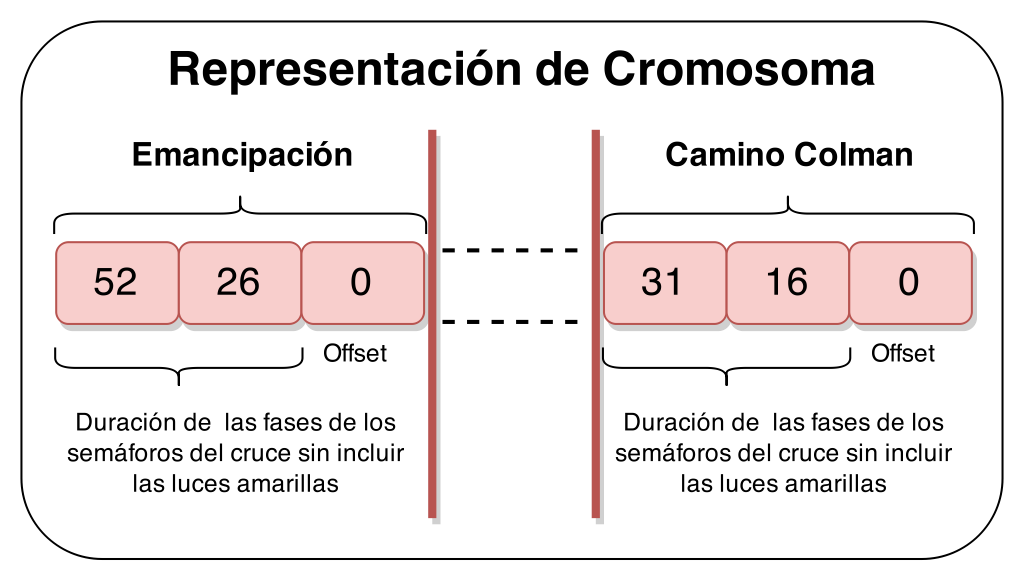
\includegraphics[width=0.7\linewidth]{Figures/cromosoma1}
 	\caption{Cromosoma de 2 cruces}
 	\label{fig:cromosoma1}
 \end{figure}
 
Es  importante que el algoritmo no genere soluciones inviables por lo que no debe modificar la combinación de luces de cada fase para evitar combinaciones de luces erróneas. Por tanto la modificación se realizará solo en el valor que indica el comienzo de fase y en los tiempos relacionados.

\begin{figure}[H]
	\centering
	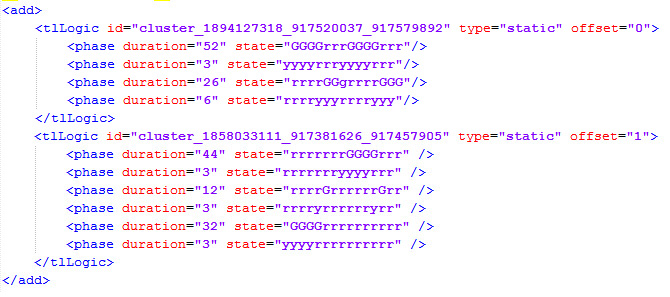
\includegraphics[width=\linewidth]{Figures/rep_sumo2}
	\caption{Representación de Sumo}
	\label{fig:rep_sumo}
\end{figure}

En la figura \ref{fig:rep_sumo} vemos el archivo con la configuración de semáforos que utiliza el simulador para el cromosoma anterior, donde se representan las fases. Por ejemplo el estado \emph{GGGGrrrGGGGrrr} indica la secuencia de luces y su duración de 52 segundos. \emph{G} indica la luz verde, \emph{r} la roja, \emph{y} el Amarillo. El \emph{offset} indica el inicio de la fase. 

En la figura \ref{fig:sem_numerados} se numeran los semáforos que se corresponden con la primera fase de este ejemplo, donde cada posición de la secuencia \emph{estado} se corresponde a un color en particular. 

\newpage
Por tanto para \emph{GGGGrrrGGGGrrr} tenemos que:
\begin{itemize}
\item GGGG se corresponde a 1, 2, 3 y 4. 
\item rrr a 5, 6 y 7. 
\item GGGG a 8, 9, 10 y 11. 
\item rrr a 12, 13 y 14. 
\end{itemize}
  
\begin{figure}[H]
	\centering
	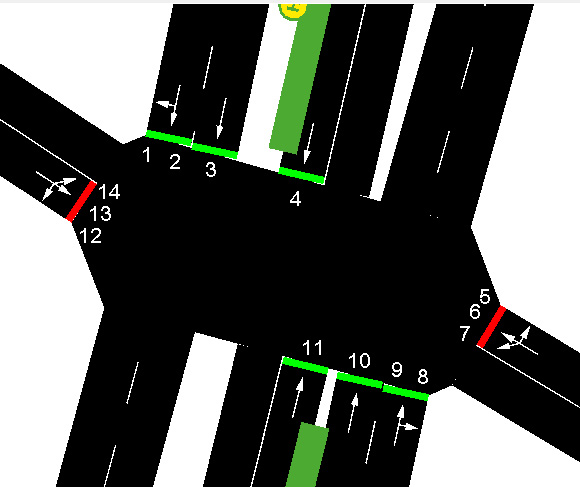
\includegraphics[width=0.7\linewidth]{Figures/semaforos_numerado}
	\caption{Representación de una fase de los semáforos para un cruce. Cada número se corresponde a una letra en la secuencia de \emph{state} del archivo de configuración del simulador SUMO.}
	\label{fig:sem_numerados}
\end{figure}

\subsection{Población inicial}

Para la inicialización de la población se toma como referencia
la configuración obtenida con los datos in-situ, luego para cada
cruce se hacen variar las duraciones de las fases de manera aleatoria entre un rango de valores configurable. Se elige la fase inicial aleatoriamente entre la cantidad de fases del cruce.

\subsection{Función \emph{fitness}}


La evaluación de un individuo se realiza generando un archivo con la configuración de los semáforos en base a su cromosoma y ejecutando el simulador SUMO utilizando esta configuración para luego obtener los datos necesarios para calcular el fitness.

Se empleará una función multiobjetivo usando combinación lineal de la velocidad de los ómnibus y del resto de los vehículos, ya que es un método sencillo y adecuado cuando son menos de tres objetivos. El \emph{fitness} se calcula como una suma ponderada, con los pesos fijados a priori.

        \begin{equation}
        \label{eq:funcion_fitness_generica}
		F(x) = \sum_{i=1}^{n}{w_i}{f_i}(x)
        \end{equation}

Se selecciona como objetivo la velocidad promedio de los ómnibus (vpb) y la velocidad promedio del resto de los vehículos (vpv). Esta métrica fue elegida pues es más adecuada para realizar las comparaciones con la realidad. Por ejemplo la cantidad de vehículos que completan su viaje, la duración promedio del recorrido o el tiempo de simulación son todas métricas que podrían usarse pero no son útiles a la hora de comparar.

Esta es la formula de fitness utilizada donde \emph{x} e \emph{y} indica el peso que le vamos a especificar a la función. 

        \begin{equation}
        \label{eq:funcion_fitness}
        f = x.vpb + y.vpv
        \end{equation}
        
En una primera instancia se establece x = y = 1 más adelante se experimentará con otros pesos.

Al apuntar a optimizar la velocidad promedio de los vehículos hay q tener en cuenta que es en toda la red, esto quiere decir que se busca una mejor velocidad promedio tanto en autos que van por Garzón como aquellos que realizan los cruces. Esto es fundamental ya que si se optimiza individualmente una calle podría traer problemas de congestión en otras zonas.

\subsection{Operadores}
\subsubsection{Operador de Cruzamiento}
Se  utilizará cruzamiento de un punto, seleccionando del cromosoma una posición aleatoria entre dos cruces como punto de corte, por tanto si un tramo del corredor tiene un buen comportamiento se intentará mantener esta propiedad.

En el escenario que se plantea en la siguiente figura, los padres cuentan con tres cruces. Se elige un punto de corte aleatoriamente entre dos cruces y se generan los hijos que son una combinación de los padres.

\begin{figure}[H]
	\centering
	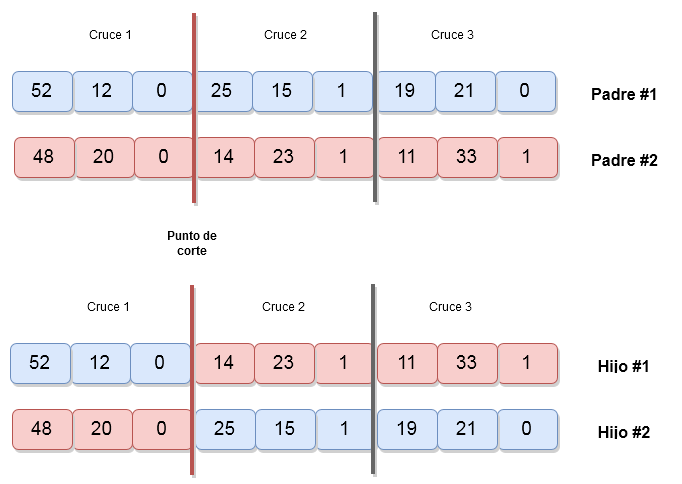
\includegraphics[width=8cm]{Figures/alg_cruzamiento}
	\caption{Visualización del cruzamiento entre individuos.}
	\label{fig:op_cruzamiento}
\end{figure}



\subsubsection{Operador de Mutación}
Se implementaron dos tipos de mutación:
\begin{itemize}

\item Mutación de duración de fase: para cada fase de cada cruce se hace variar su duración sumando o restando una cantidad dada de segundos entre un rango determinado con una probabilidad dada. Teniendo en cuenta de que el valor obtenido este dentro de un rango para que no se produzcan casos irreales como un cruce de menos de 5 segundos.

\item Mutación del \emph{offset}: Se elige aleatoriamente una fase con la cual va a comenzar inicialmente el cruce con una probabilidad dada.
\end{itemize}

\subsubsection{Operador de selección y reemplazo}
Se  utilizan los operadores provistos por el algoritmo newGA de Malva. La selección de padres se realiza por el método de torneo de tres individuos y la selección de hijos por el método de ruleta. La política de reemplazo indica que tanto padres como hijos pueden ser parte de la siguiente generación (no solamente los hijos), por lo que existe reemplazo de padres por hijos.

\subsubsection{Parámetros del algoritmo}
Los parámetros específicos del algoritmo se establecen en la siguiente sección, donde se realiza un análisis experimental para encontrar los más adecuados. Estos parámetros son: número de generaciones, tamaño de población, probabilidad de cruzamiento y de mutación.